\section{Testing and Results}
\label{sec:test}

\subsection{Testing Methodology}

Tests were ran using the SeARCH cluster, particularly the 601 and 611 nodes.

\begin{table}[!htp]
	\begin{tabular}{ll}
		\hline
		Processors per node: & 2	\\
		Processor model: & Intel\textregistered Xeon\textregistered X5650\\
		Cores per processor: & 6	\\
		Threads per core: & 2	\\
		Clock frequency: & 2.66 GHz	\\
		\hline
		L1 cache: & 32 KB + 32 KB per core	\\
		L2 cache: & 256 KB per core	\\
		L3 cache: & 12 MB shared	\\
		RAM: & 12 GB	\\
		\hline
	\end{tabular}
	\caption[SeARCH Group 601 hardware description]{SeARCH Group 601 hardware description.}
	\label{tab:group601}
\end{table}

The biggest test case used consisted of $2^{27}$ integer elements, distributed equally across each process/thread. However, MPI tests frequently crashed for big inputs (starting at $2^{19}$), probably due to buffering problems handling big amounts of large packets.

OpenMP was tested on a single node for 4, 8, and 16 threads. MPI was tested for 4 and 8 processes on a single node, 16 and 32 processes using 2 nodes (with load balancing enabled), and 64 processes across 3 nodes. SeARCH availability limitations prevented testing with a larger amount of nodes of this type. Some other tests were however ran on the 101 nodes, using up to 16 nodes.

Some variation was also introduced in the $g$ variable, controlling the number of buckets for each iteration. It was tested for values of 2, 4 and 8. However, in the interest of simplification, only the results with $g=4$ will be considered here, as the others didn't actually prove advantageous.

\subsection{Results}

After testing started, some hidden problems were found in the implementation. When the processes were distributed across more than 1 node, some errors started appearing in the larger test cases. However, due to time limitations and difficulty in debugging the application under this conditions, a fix was not found. This largely restricted the results, as only the tests that used only a single node were able to run correctly. In some, somewhat rare cases, some tests would finish correctly for multiple nodes, mas this was not very frequent and the lack of good amounts of results suggested it was better not to include them in the report.

\subsubsection{OpenMP}

\begin{figure}[!htpb]
	\begin{center}
	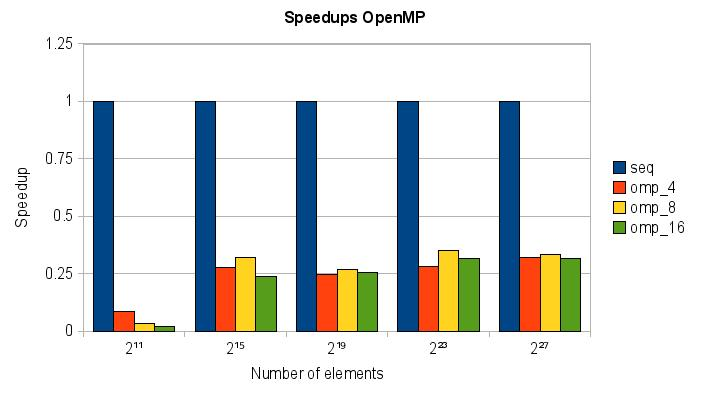
\includegraphics[width=\columnwidth]{images/speedup_omp}
	\end{center}
	\caption{OpenMP speedups}
	\label{fig:speedup_omp}
\end{figure}

\autoref{fig:speedup_omp} shows the speedup comparison for the OpenMP implementation. It was clearly unsuccessfull in bringing performance improvements. This was most likely due to the way the array is iterated. Since tasks are not homogeneous, caching is not being taken advantage of, since each thread iterates the array at a different speed. Also, for 16 threads, multithreading is enabled, since only 12 cores are available. This explains the even bigger performance drop for that version.

\subsubsection{MPI}


\begin{figure}[!htpb]
	\begin{center}
	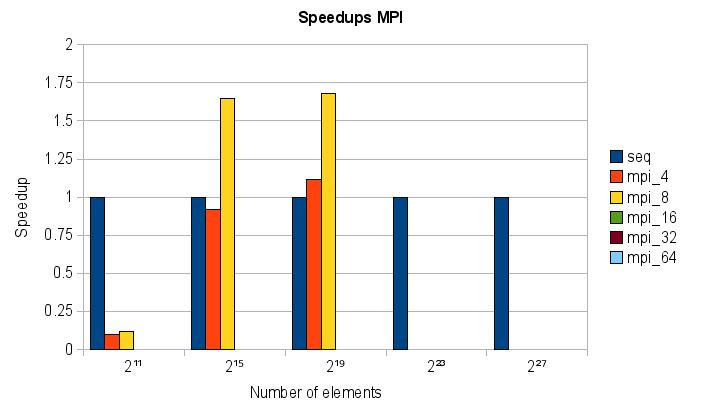
\includegraphics[width=\columnwidth]{images/speedup_mpi}
	\end{center}
	\caption{MPI speedups}
	\label{fig:speedup_mpi}
\end{figure}

\begin{figure}[!htpb]
	\begin{center}
	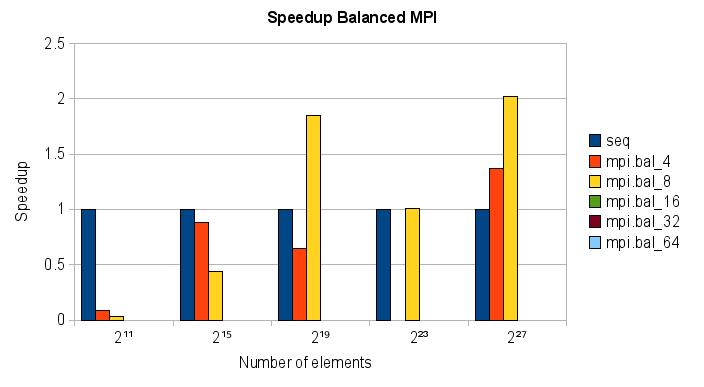
\includegraphics[width=\columnwidth]{images/speedup_mpi_bal}
	\end{center}
	\caption{Balanced MPI speedups}
	\label{fig:speedup_mpi_bal}
\end{figure}

\autoref{fig:speedup_mpi} and \autoref{fig:speedup_mpi_bal} show the small amount of MPI results that were able to be tested successfully. All the results shown were ran on a single node, and some speedups are noticeable. It can also be seen that the load balance approach only starts to be useful when the test case is big enough, although the already mentioned implementation problems hindered any advancements in thi conclusion.
